\documentclass[11pt, a4paper]{article}

\usepackage{graphicx} 
\usepackage[utf8]{inputenc}
\usepackage{fancyhdr}
\usepackage{changepage}
\usepackage[onehalfspacing]{setspace}
\usepackage{ragged2e}
\usepackage{ amssymb, amsmath, amsthm, dsfont }
\usepackage[width = 18cm, top = 2.5cm, bottom = 3cm]{geometry}
\usepackage{extarrows}
\usepackage{graphicx,color,curves,epsf,float,rotating}
% --------- Variabel, auf jedem Blatt ändern!
\newcommand{\blattnummer}{1}
\newcommand{\datum}{1. Mai 2017}
	% Punktezahlen & Summe
\newcommand{\p}{16}
\newcommand{\pp}{4}
\newcommand{\ppp}{}
\newcommand{\pppp}{}
\newcommand{\sump}{20}
% --------- Macros

\newcommand{\myTitleString} {}
\newcommand{\myAuthorString} {}
\newcommand{\mySubTitleString} {}
\newcommand{\myDateString} {}

\newcommand{\myTitle}[1] {\renewcommand {\myTitleString}{#1}}
\newcommand{\mySubTitle}[1] {\renewcommand {\mySubTitleString}{#1}}
\newcommand{\myAuthor}[1] {\renewcommand{\myAuthorString}		{#1}}
\newcommand{\myDate}[1] {\renewcommand{\myDateString}{#1}}

\newcommand{\makeMyTitle}
{
\pagestyle{fancy}
\fancyhead[L]
{
\begin{tabular}{l}
\myTitleString
\\ \mySubTitleString 
\\ \myDateString
\end{tabular}
} 			
\fancyhead[C]{}
\fancyhead[R]{\myAuthorString}
\fancyfoot[C]{\thepage}
}

\setlength{\headheight}{45pt}

\makeatletter
\renewcommand*\env@matrix[1][*\c@MaxMatrixCols c]{%
  \hskip -\arraycolsep
  \let\@ifnextchar\new@ifnextchar
  \array{#1}}
\makeatother

	% args: Aufgabennummer, erreichbare Punkte
\newcommand{\aufgabe}[2] {\section*{Aufgabe \blattnummer.#1 (Punkte:\qquad/#2)}}
\newcommand{\aufgabenteil}[1] {\textbf{(#1)}}
% ---------
%\setlength{\parindent}{0pt}
\begin{document}

\myTitle{\textsc{Datenbanken und Informationssysteme}}
\mySubTitle{Übung \blattnummer}
\myDate{\datum}
\myAuthor
{
\begin{tabular}{l l}
359109, &Michelle Milde\\
356148, &Philipp Hochmann\\
356092, &Daniel Schleiz
\end{tabular}
}
\makeMyTitle

\hfill
\begin{tabular}{|c|c|c|}\hline
   1.1 & 1.2 & $\sum$\\\hline
  	 \qquad/\p & \qquad/\pp & \qquad/\sump\\\hline % abhängig vom Übungsblatt
 \end{tabular}
\hfill Korrigiert am:\underline{\hspace{3cm}}
\hfill
\vspace*{30pt}


\aufgabe{1}{\p}
\begin{figure}[H]
  \centering
  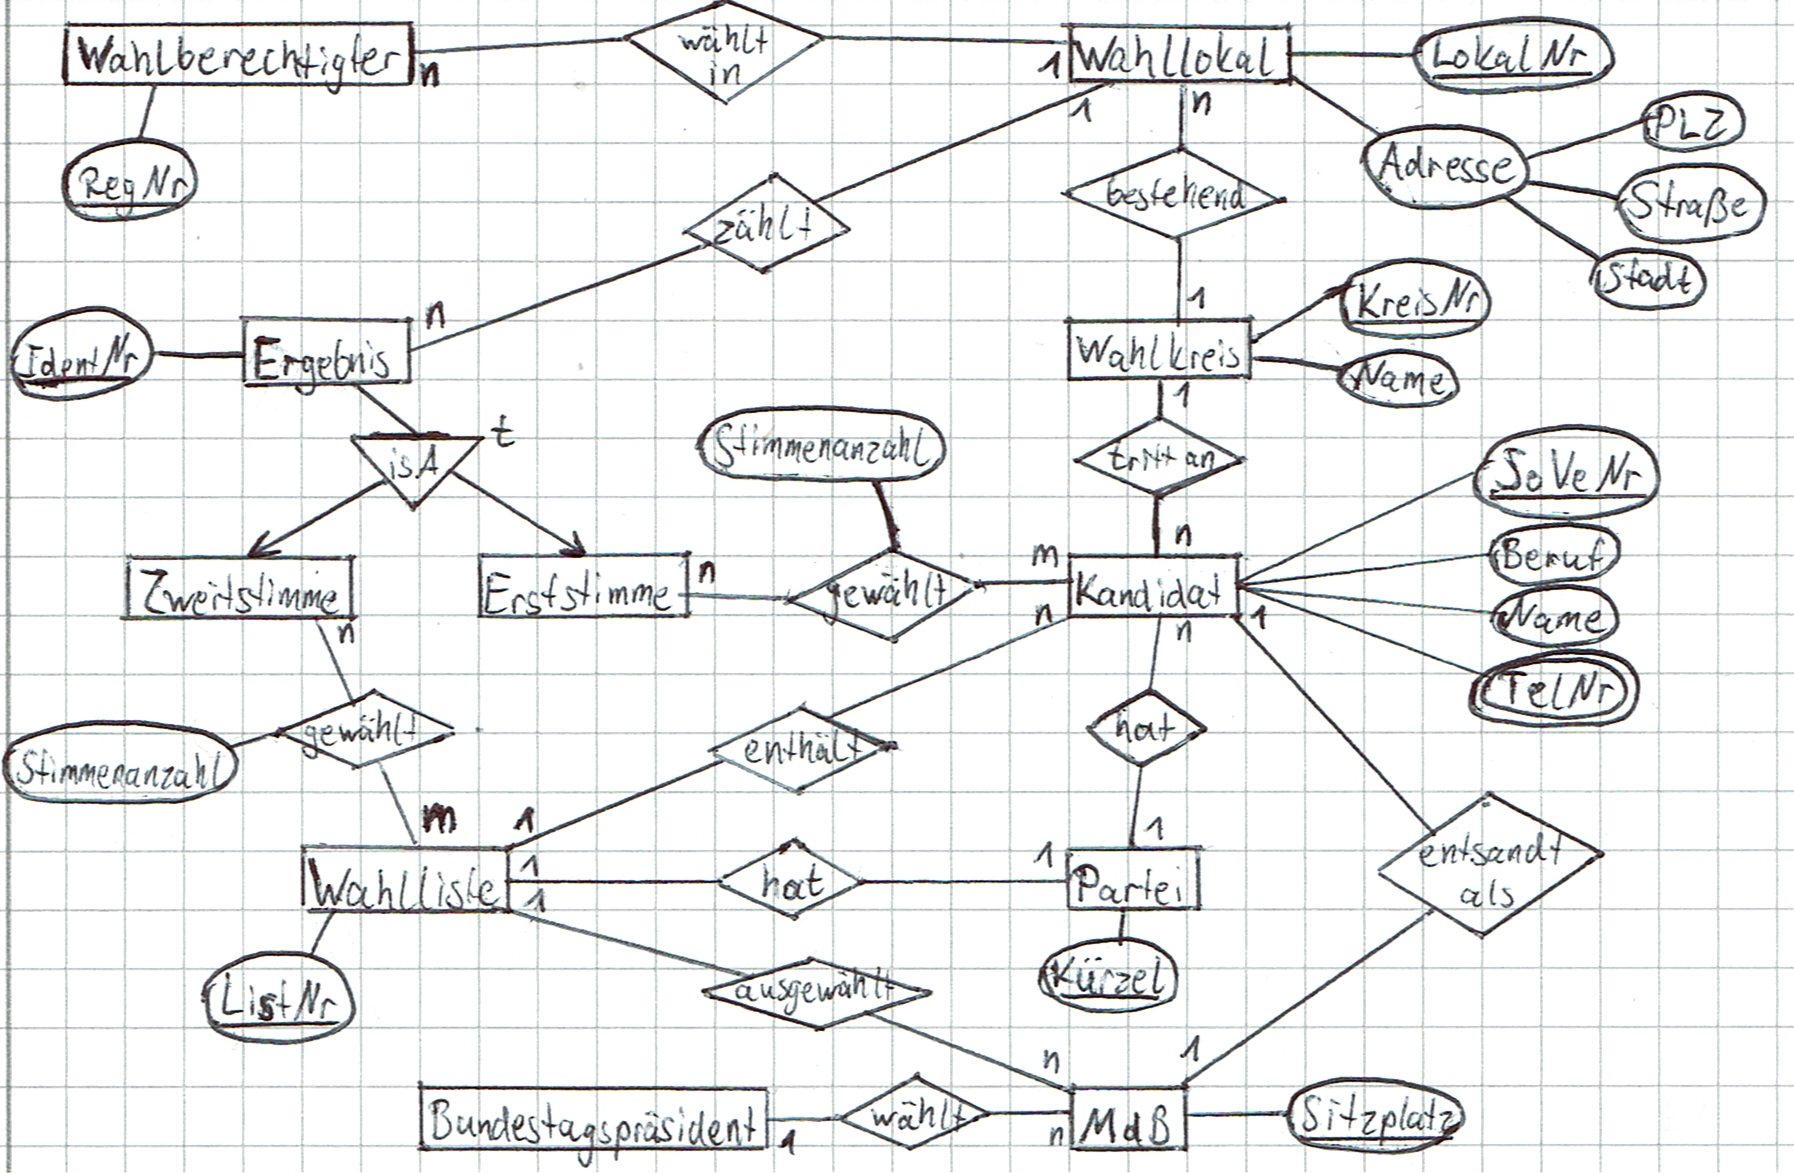
\includegraphics{a1.png}
\end{figure}\


\aufgabe{2}{\pp}
\begin{figure}[H]
  \centering
  \scalebox{.62}{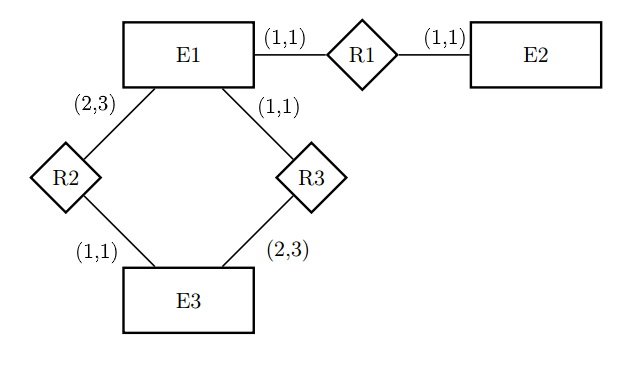
\includegraphics{a2.png}}
\end{figure}
\begin{adjustwidth}{20pt}{20pt}
Dieses ER-Diagramm ist inkonsistent, denn: \par
Jede Entity vom Typ E1 steht mit genau einer Entity vom Typ E3 in Relation (R3) , während jedes E3 mit minimal 2 und maximal 3 E1 in Relation R3 steht.
Daraus folgt, dass mindestens 2 Mal (und maximal 3 Mal) so viele E1 wie E3 benötigt werden, die wie beschrieben in Relation R3 stehen. \par
Betrachte nun die Relation R2: Für diese gilt genau das Umgekehrte, d.h. dass mindestens 2 Mal (und maximal 3 Mal) so viele E3 wie E1 benötigt werden.
Dies führt zu einem Widerspruch, außer für die leere Menge von Entities (und Relationships), oder für eine unendlich große Anzahl von E1 und E3 Entities.
Somit ist das ER-Diagramm inkonsistent.

\end{adjustwidth}



% ----------
\end{document}
